\subsection{Propuesta Definición}

\frame{
  \frametitle{Propuesta-Definición}
Y una vez repasado el estado del arte...


\begin{figure}[htb]
\centering
	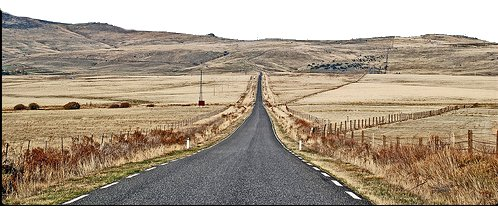
\includegraphics[width=6cm]{images/punto-partida}
\caption{Comienza nuestro camino.}

\end{figure}

}


\frame{
  \frametitle{Definición}

\begin{block}{En pocas palabras...}

\begin{itemize}[<+->]
\item Uso de un modelo conceptual de dominio (MCD).
\item Unificación de los distintos modelos de datos.
\item Descripción de los servicios de acuerdo a este modelo común.
\item Creación de plantillas BPEL que se rellenan automáticamente con la
información de los servicios y se exponen como servicios dentro del ESB.
\item Entorno controlado para el despliegue y ejecución de servicios (ESB+BPEL).
 
\end{itemize}

 
\end{block}

}


\frame{
  \frametitle{Definición}

\begin{exampleblock}{Puntos diferenciadores:}

\begin{enumerate}[<+->]
\item La semántica actúa sobre los servicios como una capa superior que es
capaz de generar código siguiendo un estándar, BPEL. En WSMO la semántica está
implícita en todos los componentes de su plataforma de ejecución.

\item La ejecución es delegada a productos comerciales perfectamente probados,
ESB+BPEL \textit{engine}. En la propuesta de WSMO han implementado desde cero y
por completo una solución (WSMX).
 
\end{enumerate}

 
\end{exampleblock}

}

\subsection{Propuesta-Infraestructura}
\frame{
  \frametitle{Infraestructura}

\begin{block}{Infraestructura}

\begin{itemize}
 \item WSMX (no funcional).
 \item Un orquestador para BPEL (hay que desplegar más componentes).
 \item OSGi (sólo para Java y no BPEL).
 \item Una \textit{suite} comercial, por ejemplo OracleSOA (coste).
 \item Un ESB \textit{open source} con soporte para BPEL. 
\end{itemize}
 
\end{block}

}


\frame{
  \frametitle{Infraestructura}

\begin{alertblock}{Infraestructura-JBoss
ESB~\footnote{\url{http://www.jboss.com/products/platforms/soa/}}}


\begin{itemize}
 \item Sigue los estándares de OASIS y W3C.
 \item Versión libre y comercial.
 \item Soporte reglas de negocio: Drools.
\item Parte de una \textit{suite} de
\textit{frameworks}\footnote{\url{http://www.jboss.org/projects/matrix}}.
\end{itemize}

 
\end{alertblock}


}


\frame{
  \frametitle{Infraestructura}

\begin{figure}[htb]
\centering
	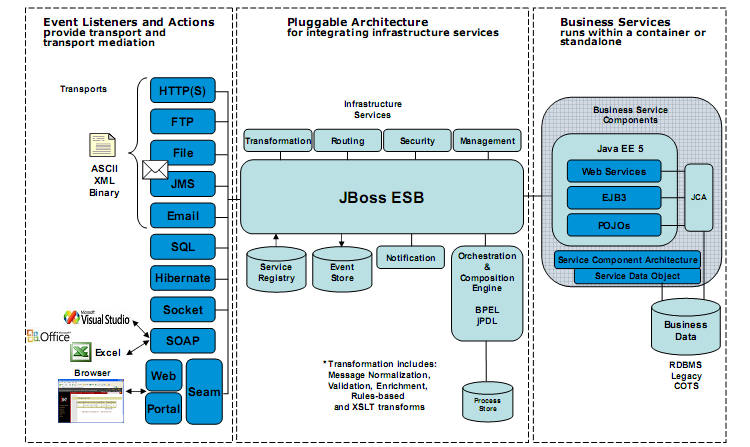
\includegraphics[width=8cm]{images/jboss-soa}
\caption{JBoss SOA.}
\end{figure}


}


\frame{
  \frametitle{Arquitectura}

Al igual que en WSMO, SUPER Project o SOA4All...

\begin{alertblock}{Arquitectura basada en componentes}

\begin{itemize}
 \item Componentes desacoplados.
 \item Estandarización de la comunicación. (WSDL+SOAP).
\end{itemize}

 
\end{alertblock}
}

\subsection{Propuesta-Análisis}
\frame{
  \frametitle{Análisis}

\begin{block}{Requisitos Funcionales~\footnote{Ver Tabla 7.1 en página 67.}
(resumen)}

\begin{itemize}
 \item Creación de un MCD.
 \item Gestión de servicios de acuerdo al MCD.
 \item Soporte para \textit{grounding} de datos.
 \item Soporte para mediación de datos.
 \item Soporte para orquestación y composición de servicios.
 \item Soporte para la ejecución de servicios.
 \item \ldots
\end{itemize}

 
\end{block}




}

\frame{
  \frametitle{Análisis}

\begin{block}{Requisitos No Funcionales~\footnote{Ver Tabla 7.2 en la página
68.} (resumen)}

\begin{itemize}
 \item Seguridad.
 \item Monitorización.
 \item Consola de administración.
 \item Facilidad de mantenimiento.
 \item Documentación multiperfil.
 \item \ldots
\end{itemize}

 
\end{block}


}


\frame{
  \frametitle{Análisis}

Vista preliminar de la arquitectura.


\begin{figure}[htb]
\centering
	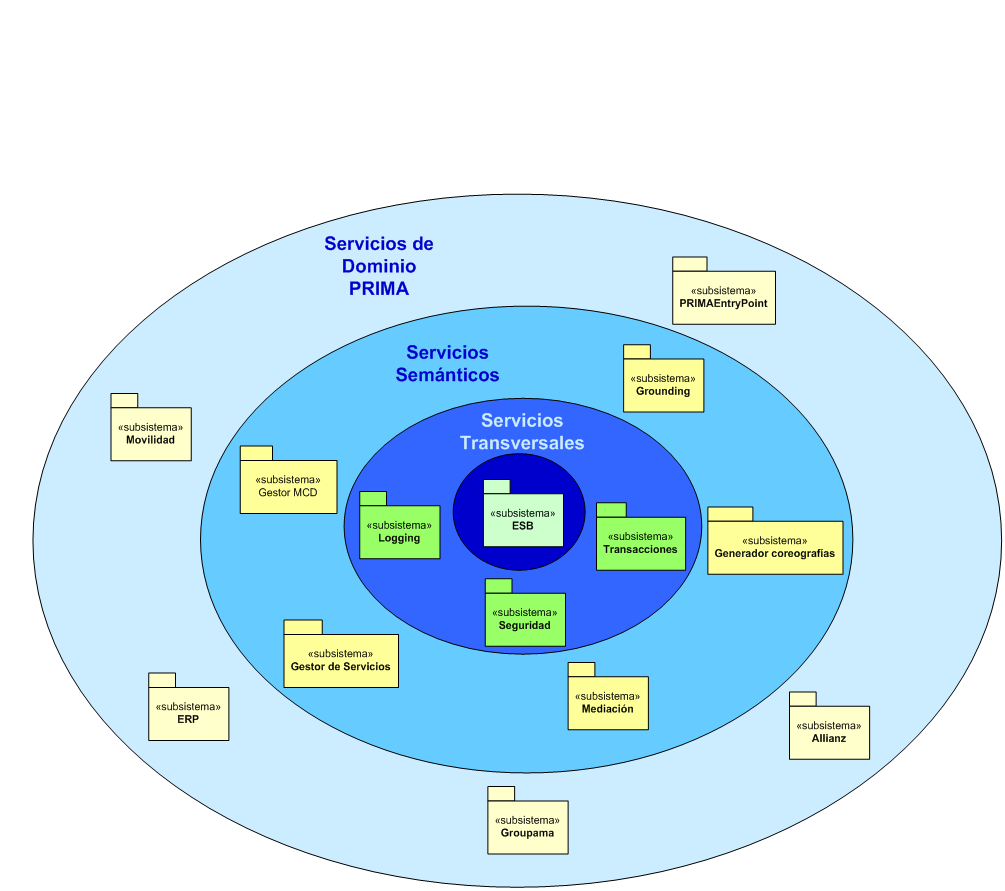
\includegraphics[width=6cm]{images/prima-capas}
\caption {Arquitectura en Capas (tomada de la documentación del proyecto
PRIMA).}
\label{fig:prima-capas}
\end{figure}

Todos los requisitos están alineados con los componentes (ver Tabla 7.3 en
la página 70).

}


\frame{
  \frametitle{Análisis}

Vista de la arquitectura en bloques.


% 
% 
\begin{figure}[h!]
\centering
	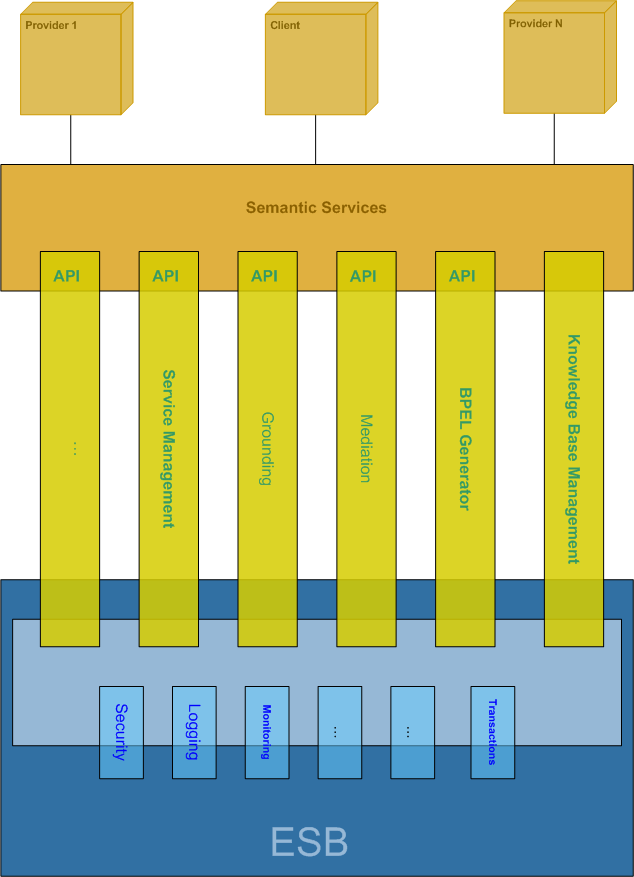
\includegraphics[width=4cm]{images/components}
\caption{Arquitectura en Bloques (presentado en ICWE2009).}
\label{fig:prima-bloques}
\end{figure}

}





\frame{
  \frametitle{Análisis}

\begin{block}{Servicios de Infraestructura}
 \begin{enumerate}[<+->]
  \item Gestión de MCD. Alta, baja y consulta del MCD.
  \item  \textit{Grounding}. Ejecución del componente de
\textit{grounding}. 
 \item Mediación. Ejecución del componente de mediación.
 \item Gestor de Servicios.  Alta, baja y consulta de la información de los
servicios técnicos.
 \item Generación de código BPEL. Genera procesos de negocio mediante la
información provista en el MCD y los servicios técnicos disponibles.
\item Despliegue de los procesos de negocio BPEL. Despliega el proceso de
negocio.

 \end{enumerate}

\end{block}
}

\frame{
  \frametitle{Análisis}

\begin{block}{Servicios de Negocio y Técnicos}
 \begin{enumerate}[<+->]
  \item Procesos de negocio. Servicios de alto nivel, vista de negocio.
  \item Servicios de técnicos de negocio. Son los servicios que proveen
operaciones para implementar procesos de negocio.
 \end{enumerate}
\end{block}
}
%Componente a componente

\frame{
  \frametitle{Análisis}

\begin{exampleblock}{Común a todos los componentes}
 \begin{itemize}
  \item Interfaz de gestión. Diseño en JMX.
  \item Interfaz de operaciones. Diseño de WSDL+SOAP.
  \item Despliegue distribuido. Por ejemplo: WAR, JBI, .Net web service.
  \item Selección del lenguaje de implementación (independiente). Según
necesidades: Java, .Net, Python, etc.
 \item Persistencia (si fuera necesario): BB.DD. relacionales o
\textit{RDF-Stores}.
 \item Ámbito: todos necesarios en tiempo de ejecución.
 \end{itemize}
\end{exampleblock}
}



\frame{
  \frametitle{Análisis}

\begin{block}{Gestor MCD}
\begin{itemize}
\item Almacenar la base de conocimiento del negocio.
\item Disponer de un modelo de datos para un sector de negocio. 
\item Describir las operaciones que se pueden realizar en el sector de negocio.
(\textit{GOALs} o servicios de negocio). 
\item Describir los servicios técnicos y de negocio. No los de infraestructura.
\end{itemize}
\end{block}
}


\frame{
  \frametitle{Análisis}

\begin{block}{Gestor de Servicios}
 \begin{itemize}
\item Listar proveedores de los servicios técnicos.
\item Añadir proveedor.
\item Listar operaciones o servicios técnicos.
\item Listar anotaciones (de acuerdo al MCD) y reglas de mapeo. Para que un
proveedor pueda ser dado
de alta debe proveer información sobre cómo realizar el \textit{grounding}.
\item Listar WSDLs por proveedor.
\item Listar operaciones por proveedor y WSDL.
\item Listar anotaciones: y reglas de mapeo por proveedor,  WSDL y anotaciones.
\item Añadir servicio técnico.
\item Ver servicio técnico.
 \end{itemize}
\end{block}
}


\frame{
  \frametitle{Análisis}

\begin{block}{Core}
 \begin{itemize}
\item Disponer información del estado de los distintos componentes.
\item Manejar de los componentes de infraestructura de la plataforma:
despliegue,
repliegue, arranque, parada y consulta de estado.
\item Desplegar de los procesos de negocio generados por el componente de
generación de código BPEL.
\item Servir como punto de entrada a los posibles clientes de los procesos de
negocio.
 \end{itemize}
\end{block}
}

\frame{
  \frametitle{Análisis}

\begin{block}{Grounding}
 \begin{itemize}
 \item Realizar el proceso de \textit{lowering}. Degradar el modelo de datos
común a cada uno de los modelos de datos particulares, generando así el
\textit{payload} de los mensajes SOAP.

\item Realizar el proceso de \textit{lifting}. Transformando el \textit{payload}
de un mensaje SOAP con un modelo de datos particular al modelo de datos común.
 \end{itemize}
\end{block}

\begin{alertblock}{Nota:}
 Este componente ha sido desarrollado por Miguel García en su proyecto fin de
máster: \textit{AGUA: Automatic Grounding Using Annotation}. Está liberado en:
~\url{http://agua.morfeo-project.org}.
\end{alertblock}
}

\frame{
  \frametitle{Análisis}
\begin{figure}[ht]
	\centering
   	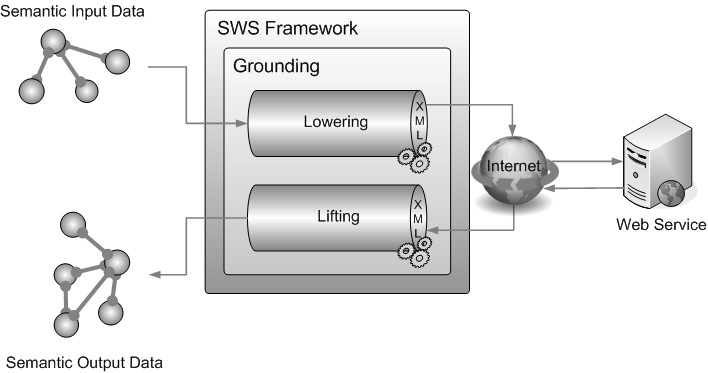
\includegraphics[width=8cm]{images/proceso-grounding}
		\caption{Ejecución de \textit{Grounding}.}
\end{figure}
}

\frame{
  \frametitle{Análisis}

\begin{block}{Mediación}
 \begin{itemize}
  \item Mediación de datos entre dos modelos de datos. Recibe: grafo de entrada,
modelo grafo de entrada, modelo grafo de salida, reglas de transformación.
Devuelve: un grafo de salida de acuerdo al modelo del grafo de salida.
 \end{itemize}
\end{block}

\begin{alertblock}{Nota:}
 Este componente, llamado \textit{DAta Mediation Adaptative}, ha sido diseñado
e implementado durante los cursos de doctorado de: ``Lenguajes dinámicos'' y
``Reflectividad''.
\end{alertblock}

}


\frame{
  \frametitle{Análisis}

\begin{block}{Generador de código BPEL}
 \begin{itemize}
  \item Generar código BPEL desde una serie de parámetros de entrada: Plantilla
del servicio de negocio a generar (un documento pseudo-BPEL), información de los
servicios técnicos, información del MCD y opcionalmente unas reglas de
generación de código.
 \end{itemize}
\end{block}
}


\frame{
  \frametitle{Propuesta-Diseño}

\begin{figure}[htb]
\centering
	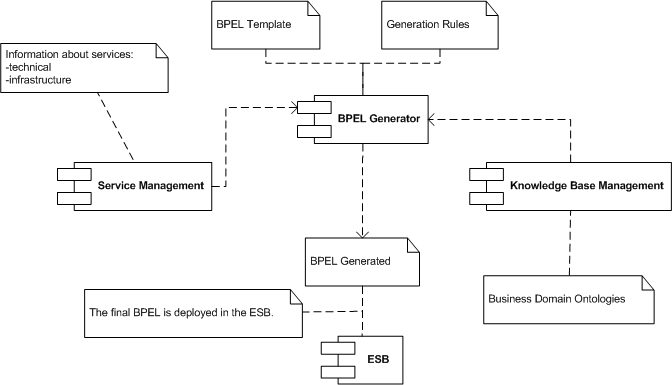
\includegraphics[width=7cm]{images/bpel-generator}
\caption{Generación de código BPEL~\footnote{Ver Figura 7.21 en página 93.}.}
\end{figure}


}

\frame{
  \frametitle{Análisis}

\begin{block}{Generador de código BPEL-Pasos de Ejecución}
 \begin{itemize}
\item Consulta al Gestor del MCD para conseguir la descripción de los servicios
de negocio. 
\item Cada servicio de negocio está formado por una serie de invocaciones a
servicios técnicos. 
\item Cada servicio técnico además de la invocación propia requiere invocaciones
a los servicios de infraestructura: \textit{grounding} y mediación.
 \end{itemize}
\end{block}
}


\frame{
  \frametitle{Análisis}

\begin{block}{Generador de código BPEL-Pasos de Ejecución II}
 \begin{itemize}

\item Cada servicio técnico recibe una entrada y devuelve una salida. Tiene un
proveedor de la operación y está especificado a través conceptos del MCD. Con lo
cual todos los servicios técnicos trabajan de forma abstracta con el mismo
modelo.
\item La información operacional del servicio técnico es extraída del Gestor de
Servicios.
\item Se repiten las operaciones hasta que se rellenen las invocaciones a todos
los servicios técnicos necesarios.
 \end{itemize}
\end{block}
}

\subsection{Propuesta-Diseño}
\frame{
  \frametitle{Diseño}

\begin{figure}[htb]
\centering
	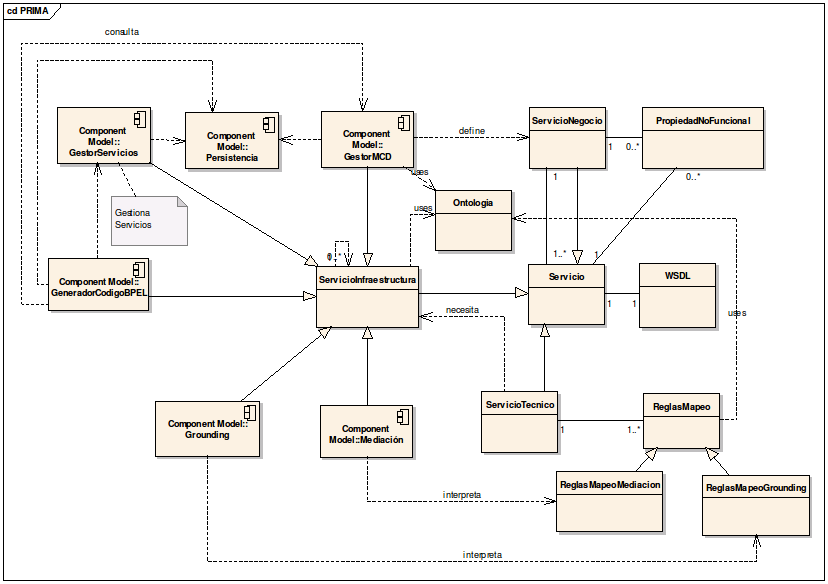
\includegraphics[width=7cm]{images/prima-componentes}
\caption{Diagrama de Clases y Componentes~\footnote{Ver Figura 7.7 en página
84.}.}
\end{figure}

}


\frame{
  \frametitle{Modelo Dinámico}

\begin{figure}[htb]
\centering
	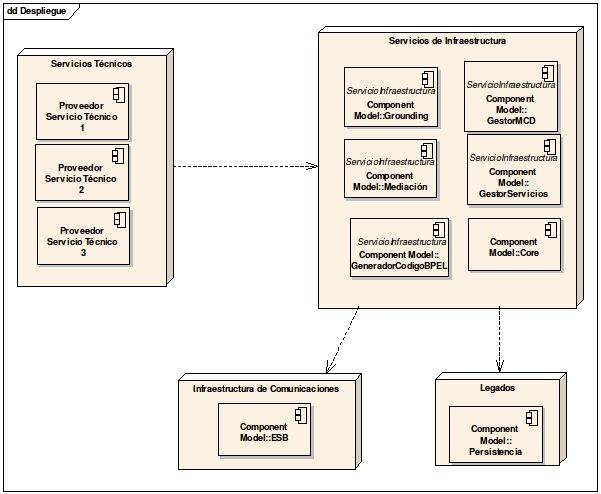
\includegraphics[width=6cm]{images/despliegue}
\caption{Diagrama de Despliegue~\footnote{Ver Figura 7.22 en página 94.}.}
\end{figure}

}


\frame{
  \frametitle{Arquitectura}


\begin{exampleblock}{Más información de la especificación}
 \begin{itemize}
  \item Diseño de operaciones. Ver páginas 78-89.
  \item Modelo dinámico. Ver página 89-93.
  \item Administración de la plataforma. Ver página 94.
  \item Requisitos de integración para terceros. Ver página 95.
  \item Otros: tests de integración, etc. Ver página 105.
 \end{itemize}
\end{exampleblock}
}


\subsection{Propuesta-Ejecución y Ejemplos}

\frame{
  \frametitle{Ejecución}

\begin{figure}[htb]
\centering
	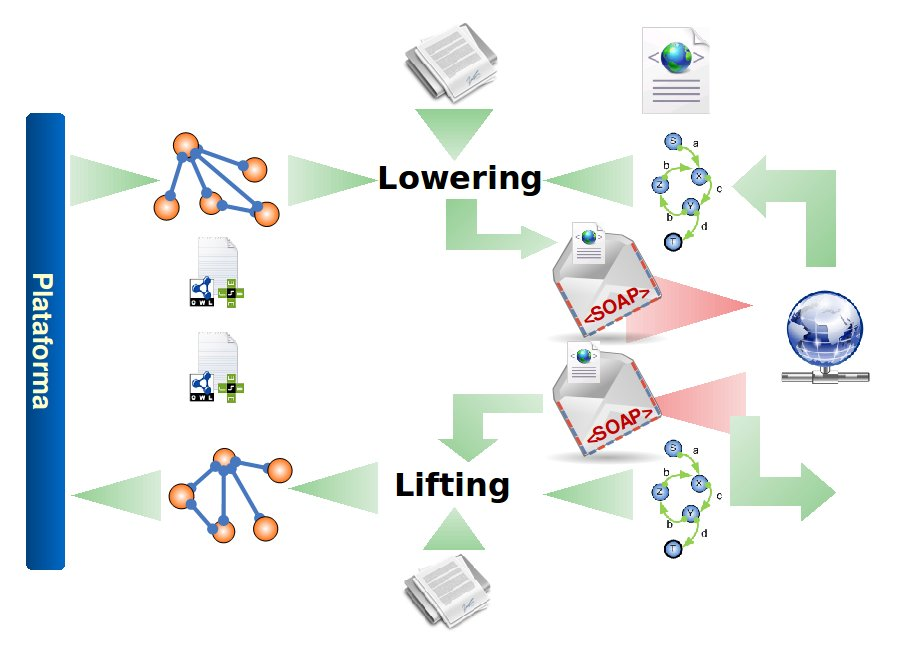
\includegraphics[width=8cm]{images/invocacion}
\caption{Ejemplo de invocación.}
\end{figure}

}


\frame{
  \frametitle{Ejemplos}

\begin{block}{Ejemplos}
\begin{itemize}
\item MCD (en WSML fácil de leer). 
\item Servicio web modelado de acuerdo al MCD.
\item Datos para petición en RDF de acuerdo al MCD.
\item Datos de respuesta en RDF de acuerdo al MCD.
\item Petición SOAP.
\item Respuesta SOAP.
\item Proceso BPEL de Multitarifación.
\end{itemize}
\end{block}

}



\frame{
  \frametitle{BPEL}

\begin{figure}[htb]
\centering
	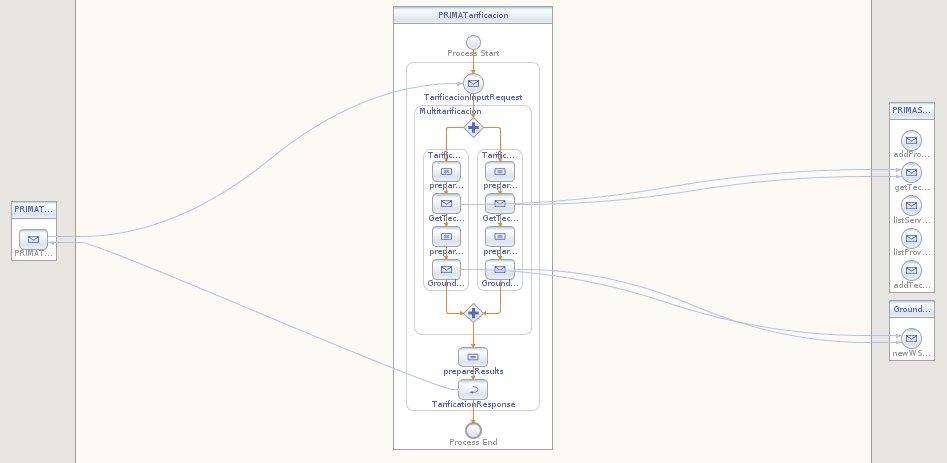
\includegraphics[width=10cm]{images/multitarificacion}
\caption{BPEL de Multitarificación~\footnote{Ver página 110.}.}
\end{figure}

}

\subsection{Propuesta-Resumen}
\frame{
  \frametitle{Resumen}

\begin{exampleblock}{Aplicación de Semántica}<1->
 \begin{itemize}
\item Toda la plataforma es guiada por un MCD.
\item Los servicios de negocio están definidos de acuerdo al MCD.
\item Los servicios técnicos están anotados usando conceptos del MCD.
\item La generación de código BPEL para el proceso de negocio se basa en el MCD
y en el gestor de servicios. Por lo tanto, tiene implícita su semántica.
 \end{itemize}
\end{exampleblock}

\begin{alertblock}{Factores diferenciadores}<2->
\begin{itemize}
\item Uso de estándares. 
\item Delegación de la ejecución a productos estables.
\end{itemize}
\end{alertblock}



}

